\underline{Photodiode}

The final part of this experiment deals with inserting a photodiode into the circuit. It should be noted that a phototransistor is used instead of a photodiode since a  phototransistor has similar characteristics as a photodiode when light is illuminated onto it, even being more sensitive to light. For this particular part, a PIN diode is used instead of a pn-junction diode because it has a wider depletion layer that helps more excited electrons be exposed to light. When light is illuminated onto a PIN diode, the diode absorbs more photons and produces more power. Photons at a high frequency excite electrons from the valence band to the conduction band since their energy level is higher than the bandgap energy. The phototransistor is to be regarded in three cases (reverse bias, zero bias, and forward bias). When electrons jump from the valence band to conduction band, the electric field in the region with a shortage of electrons cause the electrons to move in a reverse-biased direction. The reverse bias current is driven by the excited electrons, which as a result supply the load with power. The second case for this phototransistor is being zero biased. The flow of current out of the diode is restricted and a voltage builds up, which leads to some amount of power generation. For both cases of reverse bias and zero bias, the voltage drop over the diode increases as light shines on the phototransistor. The power generated by both diodes is very similar because of the widened depletion layer. The third and final case is when the diode is in forward bias. When the diode is in forward bias, the depletion layer of the diode is decreased thus not much power being generated. Therefore, the voltage drop over the phototransistor is the same when the light is both off and on. \\



\underline{10}
When working with photodiodes the best case to collect energy of light is by shining light on a photodiode. When the light is illuminated on the diode, the photons are absorbed and more power is produced compared to using electrical power. The purpose of using solar cells is too help the environment by saving electrical/mechanical energy, and using electrical energy does the opposite of that. If a PIN diode is used, it is even better since there is an intrinsic semiconductor layer between the n-type layer and p-type layer that will help excited electrons be exposed to light. \\
\begin{table}
	\centering
	\begin{tabular}{| c | c | c | c |}\hline
		& V\textsubscript{in}=-5V & V\textsubscript{in}=0 & V\textsubscript{in}=5V \\\hline
		Without Flashlight & -0.01 & 0.075 & 0.82\\\hline
		With Flashlight & 0.50 & 0.52 & 0.82 \\\hline
	\end{tabular}
\label{Voltage over Photodiode}
\ref{photodiode_table}
\end{table}

\begin{figure}[h!]
	\centering
	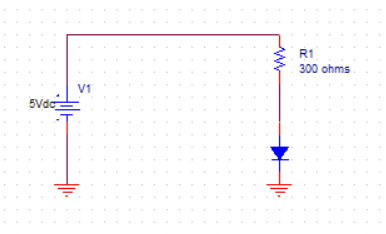
\includegraphics{CircuitSchematic.PNG}
	\caption{Experiment 4 Circuit}
	\label{fig:Circuit_Pic}
\end{figure}

